\chapter{Mesure des positions - Différents essais d'étallonage}
\label{annexe:MesPos}

\section{Introduction}
Cette annexe vient traiter les différentes approches effectuer afin de calibrer correctement les capteurs de positions.

\subsection{Première mesure des capteurs de position}
La première série d'essais correspond à la configuration matérielle issue du précédent travail de bachelor. Les résultats obtenus sont détaillés dans les tableaux \ref{tab:premier_mesure_pos_cond} et \ref{tab:premier_mesure_pos_adc} :

% --- Tableau 1 : Après le conditionnement ---
\begin{table}[H]
    \centering
    \begin{tabular}{|c|c|c|c|c|}
        \hline
        \multicolumn{5}{|c|}{\textbf{Mesure des positions après le conditionnement}}                 \\ \hline
        Inducteur          & Théorique {[}V{]} & Mesurée {[}V{]} & Erreur & Erreur relative {[}\%{]} \\ \hline
        \multirow{3}{*}{1} & 1.000             & 1.043           & 0.043  & 4.300                    \\ \cline{2-5}
                           & 2.000             & 1.982           & 0.018  & 0.900                    \\ \cline{2-5}
                           & 3.000             & 2.986           & 0.014  & 0.467                    \\ \hline
        \multirow{3}{*}{2} & 1.000             & 0.994           & 0.006  & 0.600                    \\ \cline{2-5}
                           & 2.000             & 1.939           & 0.061  & 3.050                    \\ \cline{2-5}
                           & 3.000             & 2.962           & 0.038  & 1.267                    \\ \hline
        \multirow{3}{*}{3} & 1.000             & 0.763           & 0.237  & 23.700                   \\ \cline{2-5}
                           & 2.000             & 1.769           & 0.231  & 11.550                   \\ \cline{2-5}
                           & 3.000             & 2.891           & 0.109  & 3.633                    \\ \hline
        \multirow{3}{*}{4} & 1.000             & 0.942           & 0.058  & 5.800                    \\ \cline{2-5}
                           & 2.000             & 1.913           & 0.087  & 4.350                    \\ \cline{2-5}
                           & 3.000             & 2.970           & 0.030  & 1.000                    \\ \hline
    \end{tabular}
    \caption{Première mesure des tensions en sortie de la carte de conditionnement}
    \label{tab:premier_mesure_pos_cond}
\end{table}

% --- Tableau 2 : Après l'ADC ---
\begin{table}[H]
    \centering
    \begin{tabular}{|c|c|c|c|c|}
        \hline
        \multicolumn{5}{|c|}{\textbf{Mesure des positions après l'ADC}}                                \\ \hline
        Inducteur          & Théorique {[}mm{]} & Mesurée {[}mm{]} & Erreur & Erreur relative {[}\%{]} \\ \hline
        \multirow{3}{*}{1} & 1.000              & 1.050            & 0.050  & 5.000                    \\ \cline{2-5}
                           & 2.000              & 1.989            & 0.011  & 0.550                    \\ \cline{2-5}
                           & 3.000              & 3.006            & 0.006  & 0.200                    \\ \hline
        \multirow{3}{*}{2} & 1.000              & 1.005            & 0.005  & 0.500                    \\ \cline{2-5}
                           & 2.000              & 1.945            & 0.055  & 2.750                    \\ \cline{2-5}
                           & 3.000              & 2.970            & 0.030  & 1.000                    \\ \hline
        \multirow{3}{*}{3} & 1.000              & 0.790            & 0.210  & 21.000                   \\ \cline{2-5}
                           & 2.000              & 1.786            & 0.214  & 10.700                   \\ \cline{2-5}
                           & 3.000              & 2.897            & 0.103  & 3.433                    \\ \hline
        \multirow{3}{*}{4} & 1.000              & 0.939            & 0.061  & 6.100                    \\ \cline{2-5}
                           & 2.000              & 1.907            & 0.093  & 4.650                    \\ \cline{2-5}
                           & 3.000              & 2.968            & 0.032  & 1.067                    \\ \hline
    \end{tabular}
    \caption{Première mesure des positions en sortie de l'ADC}
    \label{tab:premier_mesure_pos_adc}
\end{table}

\subsection{Mesure après la calibration du capteur 3}
À la suite de ces résultats, une première calibration par la méthode d'apprentissage "Teach-In" a été effectuée sur le capteur de l'inducteur 3. Une série de mesures, de la sortie du capteur jusqu'à l'ADC, a été réalisée afin d'analyser l'évolution de la tension. Les relevés sont présentés dans les tableaux \ref{tab:teachin_3_capteurs}, \ref{tab:teachin_3_cond} et \ref{tab:teachin_3_adc} :

% --- Tableau 1 : Après la sortie des capteurs (Droite sur l'image) ---
\begin{table}[H]
    \centering
    \begin{tabular}{|c|c|c|c|c|}
        \hline
        \multicolumn{5}{|c|}{\textbf{Mesure des positions après la sortie des capteurs}}             \\ \hline
        Inducteur          & Théorique {[}V{]} & Mesurée {[}V{]} & Erreur & Erreur relative {[}\%{]} \\ \hline
        \multirow{4}{*}{1} & 0.00              & 0.711           & 0.711  & -                        \\ \cline{2-5}
                           & 3.33              & 2.95            & 0.383  & 11.5                     \\ \cline{2-5}
                           & 6.67              & 6.2             & 0.467  & 7                        \\ \cline{2-5}
                           & 10.0              & 9.63            & 0.370  & 3.7                      \\ \hline
        \multirow{4}{*}{2} & 0.00              & 0.2034          & 0.203  & -                        \\ \cline{2-5}
                           & 3.33              & 2.687           & 0.646  & 19.39                    \\ \cline{2-5}
                           & 6.67              & 6.04            & 0.627  & 9.4                      \\ \cline{2-5}
                           & 10.0              & 9.67            & 0.330  & 3.3                      \\ \hline
        \multirow{4}{*}{3} & 0.00              & 0.2255          & 0.226  & -                        \\ \cline{2-5}
                           & 3.33              & 2.437           & 0.896  & 26.89                    \\ \cline{2-5}
                           & 6.67              & 6.02            & 0.647  & 9.7                      \\ \cline{2-5}
                           & 10.00             & 9.87            & 0.130  & 1.3                      \\ \hline
        \multirow{4}{*}{4} & 0.00              & 0.2176          & 0.218  & -                        \\ \cline{2-5}
                           & 3.33              & 2.84            & 0.493  & 14.8                     \\ \cline{2-5}
                           & 6.67              & 6.11            & 0.557  & 8.35                     \\ \cline{2-5}
                           & 10.0              & 9.87            & 0.130  & 1.3                      \\ \hline
    \end{tabular}
    \caption{Mesure des tensions en sortie des capteurs (Calibration teach-in de l'inducteur 3)}
    \label{tab:teachin_3_capteurs}
\end{table}

% --- Tableau 2 : Après le conditionneur (Milieu sur l'image) ---
\begin{table}[H]
    \centering
    \begin{tabular}{|c|c|c|c|c|}
        \hline
        \multicolumn{5}{|c|}{\textbf{Mesure des positions après le conditionneur}}                   \\ \hline
        Inducteur          & Théorique {[}V{]} & Mesurée {[}V{]} & Erreur & Erreur relative {[}\%{]} \\ \hline
        \multirow{4}{*}{1} & 0                 & 0.189           & 0.189  & -                        \\ \cline{2-5}
                           & 1                 & 0.867           & 0.133  & 13.3                     \\ \cline{2-5}
                           & 2                 & 1.88            & 0.125  & 6.25                     \\ \cline{2-5}
                           & 3                 & 2.86            & 0.138  & 4.60                     \\ \hline
        \multirow{4}{*}{2} & 0                 & 0.100           & 0.100  & -                        \\ \cline{2-5}
                           & 1                 & 0.816           & 0.184  & 18.4                     \\ \cline{2-5}
                           & 2                 & 1.84            & 0.161  & 8.05                     \\ \cline{2-5}
                           & 3                 & 2.88            & 0.119  & 3.97                     \\ \hline
        \multirow{4}{*}{3} & 0                 & 0.040           & 0.040  & -                        \\ \cline{2-5}
                           & 1                 & 0.715           & 0.285  & 28.5                     \\ \cline{2-5}
                           & 2                 & 1.82            & 0.177  & 8.85                     \\ \cline{2-5}
                           & 3                 & 2.94            & 0.059  & 1.97                     \\ \hline
        \multirow{4}{*}{4} & 0                 & 0.070           & 0.070  & -                        \\ \cline{2-5}
                           & 1                 & 0.846           & 0.154  & 15.4                     \\ \cline{2-5}
                           & 2                 & 1.86            & 0.140  & 7                        \\ \cline{2-5}
                           & 3                 & 2.94            & 0.059  & 1.97                     \\ \hline
    \end{tabular}
    \caption{Mesure des tensions en sortie du conditionneur (Calibration teach-in de l'inducteur 3)}
    \label{tab:teachin_3_cond}
\end{table}

% --- Tableau 3 : Après l'ADC (Gauche sur l'image) ---
\begin{table}[H]
    \centering
    \begin{tabular}{|c|c|c|c|c|}
        \hline
        \multicolumn{5}{|c|}{\textbf{Mesure des positions entrefers après l'ADC}}                      \\ \hline
        Inducteur          & Théorique {[}mm{]} & Mesurée {[}mm{]} & Erreur & Erreur relative {[}\%{]} \\ \hline
        \multirow{4}{*}{1} & 0.000              & 0.194            & 0.194  & -                        \\ \cline{2-5}
                           & 1.000              & 0.887            & 0.113  & 11.3                     \\ \cline{2-5}
                           & 2.000              & 1.889            & 0.111  & 5.55                     \\ \cline{2-5}
                           & 3.000              & 2.904            & 0.096  & 3.2                      \\ \hline
        \multirow{4}{*}{2} & 0.000              & 0.117            & 0.117  & -                        \\ \cline{2-5}
                           & 1.000              & 0.838            & 0.162  & 16.2                     \\ \cline{2-5}
                           & 2.000              & 1.849            & 0.151  & 7.55                     \\ \cline{2-5}
                           & 3.000              & 2.908            & 0.092  & 3.07                     \\ \hline
        \multirow{4}{*}{3} & 0.000              & 0.059            & 0.059  & -                        \\ \cline{2-5}
                           & 1.000              & 0.738            & 0.262  & 26.2                     \\ \cline{2-5}
                           & 2.000              & 1.837            & 0.163  & 8.15                     \\ \cline{2-5}
                           & 3.000              & 2.967            & 0.033  & 1.1                      \\ \hline
        \multirow{4}{*}{4} & 0.000              & 0.081            & 0.081  & -                        \\ \cline{2-5}
                           & 1.000              & 0.852            & 0.148  & 14.8                     \\ \cline{2-5}
                           & 2.000              & 1.864            & 0.136  & 6.8                      \\ \cline{2-5}
                           & 3.000              & 2.964            & 0.036  & 1.2                      \\ \hline
    \end{tabular}
    \caption{Mesure des positions en sortie de l'ADC (Calibration teach-in de l'inducteur 3)}
    \label{tab:teachin_3_adc}
\end{table}

\subsection{Premier étalonnage de chaque capteur}
Les résultats n'étant pas concluants, un étalonnage logiciel a été envisagé. L'implémentation initiale de cet étalonnage présentait plusieurs défauts : une correction par gain était bien appliquée, mais aucun décalage (offset) n'était pris en compte. De plus, les coefficients de correction destinés aux positions 1 et 2 étaient dupliqués pour les positions 3 et 4, comme l'illustre l'extrait de code suivant :

\begin{minted}{c}
// 3722.7 / 3500 = 1.06, valeur 12 bit pour 3mm / valeur mesuree ADC (2.8mm) = ecart
Position1 = (float)(ADC_pos_1) * CONV_POS2 * POS_CORRECTION_1;
// 3722.7 / 3480 = 1.07, valeur 12 bit pour 3mm / valeur mesuree ADC (2.8mm) = ecart
Position2 = (float)(ADC_pos_2) * CONV_POS2 * POS_CORRECTION_2;
Position3 = (float)(ADC_pos_3) * CONV_POS2 * POS_CORRECTION_1;
Position4 = (float)(ADC_pos_4) * CONV_POS2 * POS_CORRECTION_2;
\end{minted}

Une nouvelle procédure d'étalonnage a été mise en œuvre. Des mesures ont été effectuées sans application de la correction initiale. Seule la conversion numérique a été conservée et affichée sur l'interface web. Les valeurs mesurées sont consignées dans le tableau \ref{tab:premier_etalonnage_code_adc} :

\begin{table}[H]
    \centering
    \begin{tabular}{|c|c|c|c|c|}
        \hline
        \multicolumn{5}{|c|}{\textbf{Mesure des positions entrefers après l'ADC}}                      \\ \hline
        Inducteur          & Théorique {[}mm{]} & Mesurée {[}mm{]} & Erreur & Erreur relative {[}\%{]} \\ \hline
        \multirow{4}{*}{1} & 0.000              & 0.231            & 0.231  & -                        \\ \cline{2-5}
                           & 1.000              & 1.023            & 0.023  & 2.30                     \\ \cline{2-5}
                           & 2.000              & 1.818            & 0.182  & 9.10                     \\ \cline{2-5}
                           & 3.000              & 2.801            & 0.199  & 6.63                     \\ \hline
        \multirow{4}{*}{2} & 0.000              & 0.099            & 0.099  & -                        \\ \cline{2-5}
                           & 1.000              & 0.970            & 0.030  & 3.00                     \\ \cline{2-5}
                           & 2.000              & 1.746            & 0.254  & 12.70                    \\ \cline{2-5}
                           & 3.000              & 2.784            & 0.216  & 7.20                     \\ \hline
        \multirow{4}{*}{3} & 0.000              & 0.054            & 0.054  & -                        \\ \cline{2-5}
                           & 1.000              & 0.726            & 0.274  & 27.40                    \\ \cline{2-5}
                           & 2.000              & 1.673            & 0.327  & 16.35                    \\ \cline{2-5}
                           & 3.000              & 2.790            & 0.210  & 7.00                     \\ \hline
        \multirow{4}{*}{4} & 0.000              & 0.150            & 0.150  & -                        \\ \cline{2-5}
                           & 1.000              & 0.897            & 0.103  & 10.30                    \\ \cline{2-5}
                           & 2.000              & 1.801            & 0.199  & 9.95                     \\ \cline{2-5}
                           & 3.000              & 2.821            & 0.179  & 5.97                     \\ \hline
    \end{tabular}
    \caption{Mesure des positions en sortie de l'ADC sans correction}
    \label{tab:premier_etalonnage_code_adc}
\end{table}

Ces données ont permis d'établir les courbes présentées dans les figures \ref{fig:Prem_tracé_ind1}, \ref{fig:Prem_tracé_ind2}, \ref{fig:Prem_tracé_ind3} et \ref{fig:Prem_tracé_ind4} :

\begin{figure}[H]
    \centering
    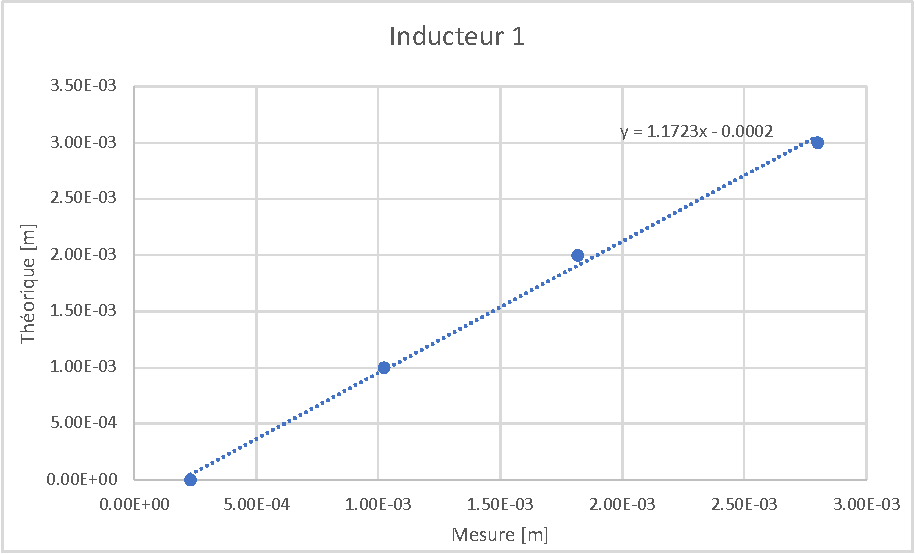
\includegraphics[width=1\linewidth]{assets/Chap3/PremEtaloInd1.pdf}
    \caption{Graphique de l'étalonnage de l'inducteur 1}
    \label{fig:Prem_tracé_ind1}
\end{figure}

\begin{figure}[H]
    \centering
    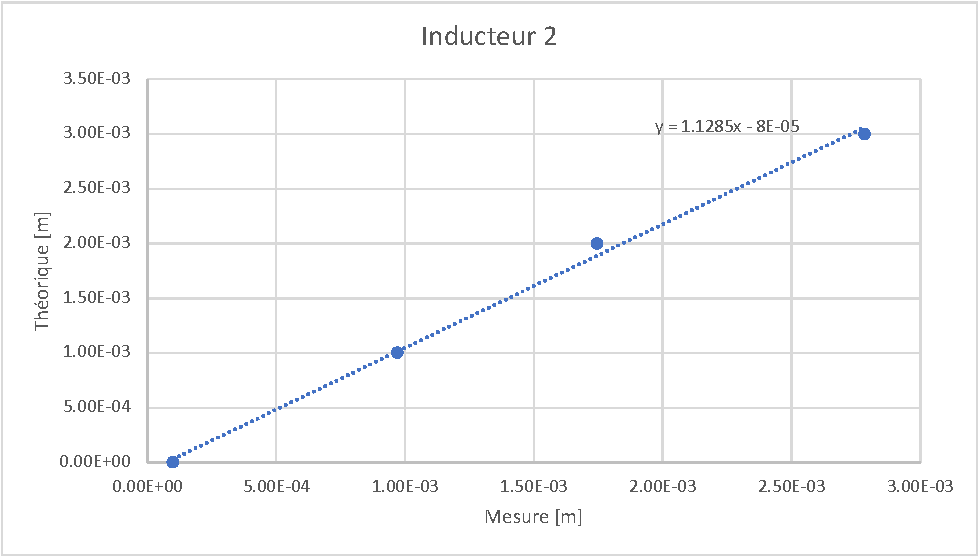
\includegraphics[width=1\linewidth]{assets/Chap3/PremEtaloInd2.pdf}
    \caption{Graphique de l'étalonnage de l'inducteur 2}
    \label{fig:Prem_tracé_ind2}
\end{figure}

\begin{figure}[H]
    \centering
    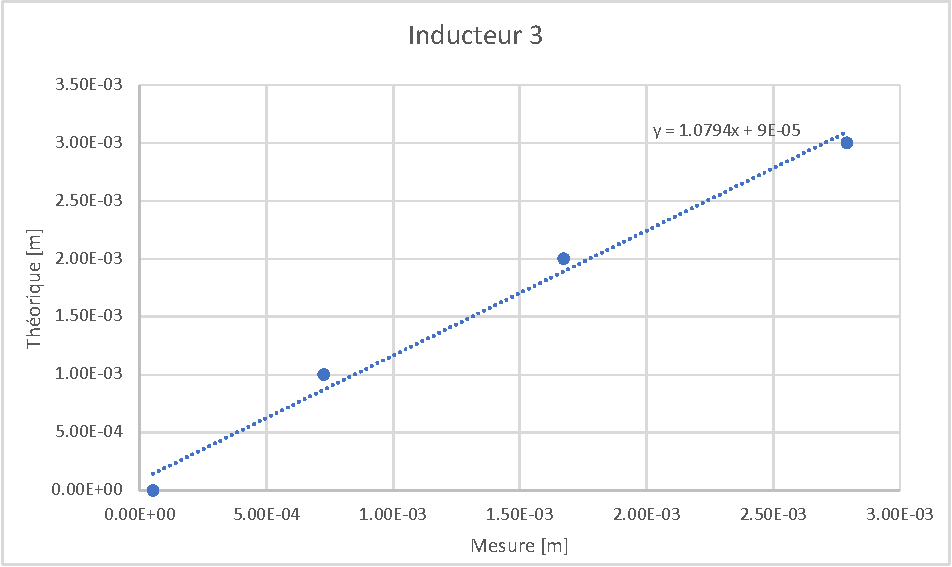
\includegraphics[width=1\linewidth]{assets/Chap3/PremEtaloInd3.pdf}
    \caption{Graphique de l'étalonnage de l'inducteur 3}
    \label{fig:Prem_tracé_ind3}
\end{figure}

\begin{figure}[H]
    \centering
    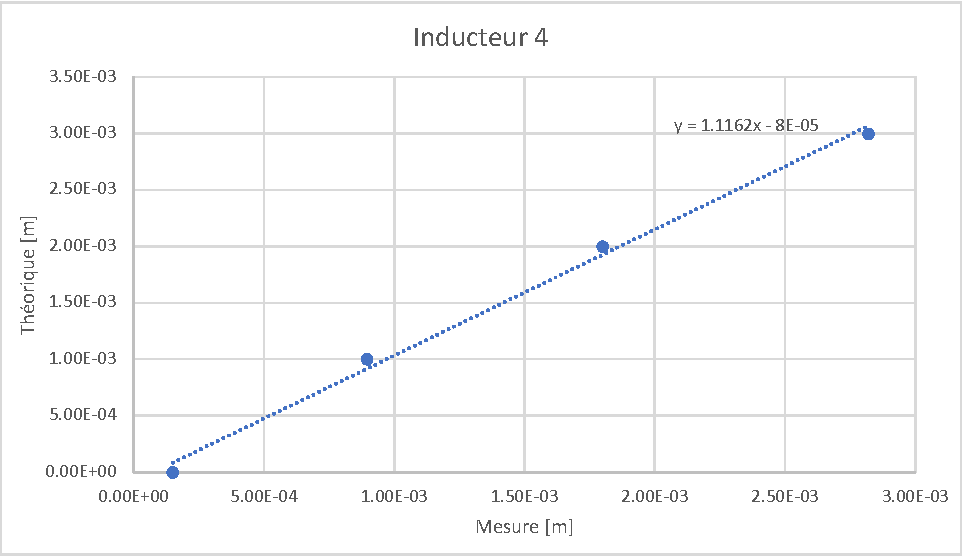
\includegraphics[width=1\linewidth]{assets/Chap3/PremEtaloInd4.pdf}
    \caption{Graphique de l'étalonnage de l'inducteur 4}
    \label{fig:Prem_tracé_ind4}
\end{figure}

L'analyse de ces tracés a permis de déduire des équations de correction intégrant un gain et un décalage (offset), où la variable $x$ représente la valeur issue de l'ADC convertie en millimètres.\\
Une vérification expérimentale a ensuite été menée, dont les résultats figurent dans le tableau \ref{tab:correction1_adc} :

\begin{table}[H]
    \centering
    \begin{tabular}{|c|c|c|c|c|}
        \hline
        \multicolumn{5}{|c|}{\textbf{Mesure des positions entrefers après l'ADC}}                     \\ \hline
        Inducteur          & Théorique {[}m{]} & Mesure {[}m{]} & Erreur   & Erreur relative {[}\%{]} \\ \hline
        \multirow{4}{*}{1} & 0.00E+00          & 1.81E-04       & 1.81E-04 & -                        \\ \cline{2-5}
                           & 1.00E-03          & 9.80E-04       & 2.00E-05 & 2.00                     \\ \cline{2-5}
                           & 2.00E-03          & 1.91E-03       & 9.10E-05 & 4.55                     \\ \cline{2-5}
                           & 3.00E-03          & 3.04E-03       & 3.90E-05 & 1.30                     \\ \hline
        \multirow{4}{*}{2} & 0.00E+00          & 1.70E-05       & 1.70E-05 & -                        \\ \cline{2-5}
                           & 1.00E-03          & 9.19E-04       & 8.10E-05 & 8.10                     \\ \cline{2-5}
                           & 2.00E-03          & 1.89E-03       & 1.07E-04 & 5.35                     \\ \cline{2-5}
                           & 3.00E-03          & 3.06E-03       & 5.80E-05 & 1.93                     \\ \hline
        \multirow{4}{*}{3} & 0.00E+00          & 1.08E-04       & 1.08E-04 & -                        \\ \cline{2-5}
                           & 1.00E-03          & 9.26E-04       & 7.40E-05 & 7.4                      \\ \cline{2-5}
                           & 2.00E-03          & 1.96E-03       & 3.70E-05 & 1.85                     \\ \cline{2-5}
                           & 3.00E-03          & 3.11E-03       & 1.09E-04 & 3.63                     \\ \hline
        \multirow{4}{*}{4} & 0.00E+00          & -1.00E-05      & 1.00E-05 & -                        \\ \cline{2-5}
                           & 1.00E-03          & 8.45E-04       & 1.55E-04 & 15.5                     \\ \cline{2-5}
                           & 2.00E-03          & 2.00E-03       & 5.00E-06 & 0.25                     \\ \cline{2-5}
                           & 3.00E-03          & 3.06E-03       & 6.10E-05 & 2.03                     \\ \hline
    \end{tabular}
    \caption{Erreurs de mesure des positions en sortie de l'ADC (1ère correction : application des courbes)}
    \label{tab:correction1_adc}
\end{table}

Malgré la faiblesse des erreurs relatives observées, l'implémentation de ces équations n'a pas apporté d'amélioration significative concernant la lévitation du système.

\subsection{Mesure après la calibration de tous les capteurs}
À la suite de l'étalonnage précédent, une calibration simultanée des quatre capteurs a été effectuée. L'objectif de cette démarche consistait à définir une origine de référence commune pour chaque inducteur :

\begin{figure}[H]
    \centering
    \includesvg[width=1\linewidth]{assets/Chap3/MaquetteCote}
    \caption{Méthode teachin en levant que l'avant}
    \label{fig:DessinMaquetteCote}
\end{figure}

Le schéma illustre le montage expérimental : le repère 7 désigne le support en bois, le repère 8 correspond à la carte principale et les repères 9 identifient les cartes de puissance.

Pour garantir une bonne homogénéité, les quatre inducteurs ont été soulevés puis abaissés selon la procédure détaillée dans la section \ref{sec:CalibrationCaptPos}.

À l'issue de cette calibration, une nouvelle série de mesures (sans correction) a été réalisée. Les données sont regroupées dans le tableau \ref{tab:recalib_sans_correction_adc} :

\begin{table}[H]
    \centering
    \begin{tabular}{|c|c|c|c|c|}
        \hline
        \multicolumn{5}{|c|}{\textbf{Mesure des positions entrefers après l'ADC}}                     \\ \hline
        Inducteur          & Théorique {[}m{]} & Mesure {[}m{]} & Erreur   & Erreur relative {[}\%{]} \\ \hline
        \multirow{4}{*}{1} & 0.00E+00          & 1.43E-04       & 1.43E-04 & -                        \\ \cline{2-5}
                           & 1.00E-03          & 8.23E-04       & 1.77E-04 & 17.7                     \\ \cline{2-5}
                           & 2.00E-03          & 1.79E-03       & 2.14E-04 & 10.7                     \\ \cline{2-5}
                           & 3.00E-03          & 2.80E-03       & 1.96E-04 & 6.53                     \\ \hline
        \multirow{4}{*}{2} & 0.00E+00          & 8.50E-05       & 8.50E-05 & -                        \\ \cline{2-5}
                           & 1.00E-03          & 8.66E-04       & 1.34E-04 & 13.4                     \\ \cline{2-5}
                           & 2.00E-03          & 1.87E-03       & 1.35E-04 & 6.75                     \\ \cline{2-5}
                           & 3.00E-03          & 2.83E-03       & 1.70E-04 & 5.67                     \\ \hline
        \multirow{4}{*}{3} & 0.00E+00          & 2.30E-05       & 2.30E-05 & -                        \\ \cline{2-5}
                           & 1.00E-03          & 7.09E-04       & 2.91E-04 & 29.1                     \\ \cline{2-5}
                           & 2.00E-03          & 1.69E-03       & 3.13E-04 & 15.65                    \\ \cline{2-5}
                           & 3.00E-03          & 2.80E-03       & 1.98E-04 & 6.6                      \\ \hline
        \multirow{4}{*}{4} & 0.00E+00          & 5.00E-05       & 5.00E-05 & -                        \\ \cline{2-5}
                           & 1.00E-03          & 8.13E-04       & 1.87E-04 & 18.7                     \\ \cline{2-5}
                           & 2.00E-03          & 1.74E-03       & 2.62E-04 & 13.1                     \\ \cline{2-5}
                           & 3.00E-03          & 2.82E-03       & 1.84E-04 & 6.13                     \\ \hline
    \end{tabular}
    \caption{Mesure des positions en sortie de l'ADC après recalibration complète et sans correction}
    \label{tab:recalib_sans_correction_adc}
\end{table}

Ces nouvelles données ont fait l'objet d'une modélisation graphique afin d'en déduire une fonction de correction à implémenter au sein du microcontrôleur. Les courbes obtenues sont visibles sur les figures \ref{fig:Sec_tracé_ind1}, \ref{fig:Sec_tracé_ind2}, \ref{fig:Sec_tracé_ind3} et \ref{fig:Sec_tracé_ind4} :

\begin{figure}[H]
    \centering
    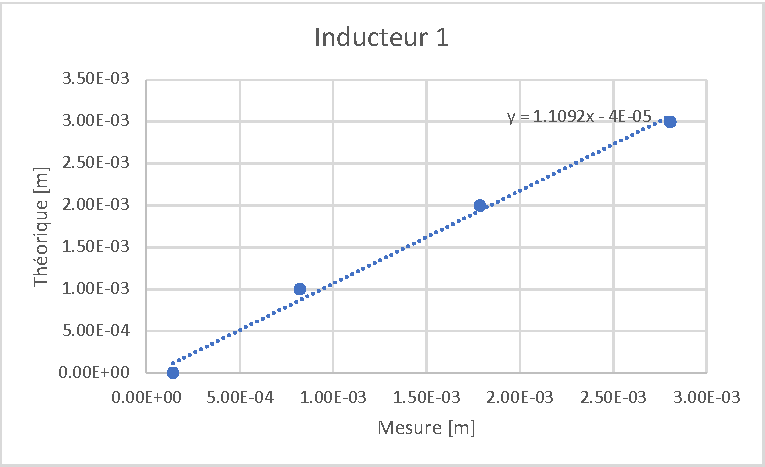
\includegraphics[width=1\linewidth]{assets/Chap3/SecEtaloInd1.pdf}
    \caption{Graphique du second étalonnage de l'inducteur 1}
    \label{fig:Sec_tracé_ind1}
\end{figure}

\begin{figure}[H]
    \centering
    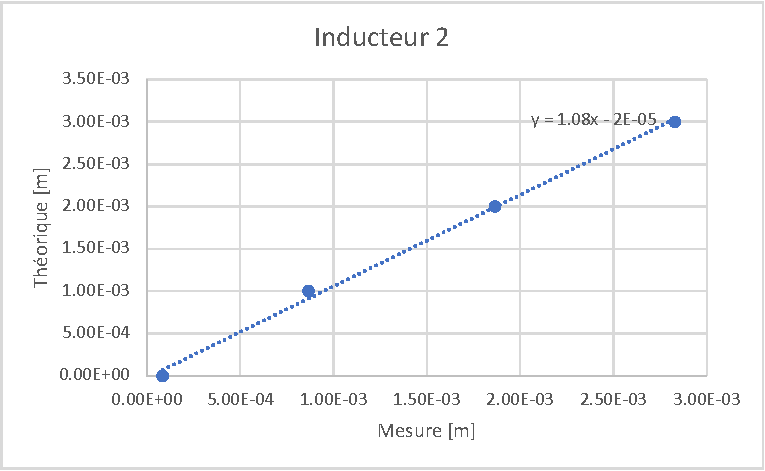
\includegraphics[width=1\linewidth]{assets/Chap3/SecEtaloInd2.pdf}
    \caption{Graphique du second étalonnage de l'inducteur 1}
    \label{fig:Sec_tracé_ind2}
\end{figure}

\begin{figure}[H]
    \centering
    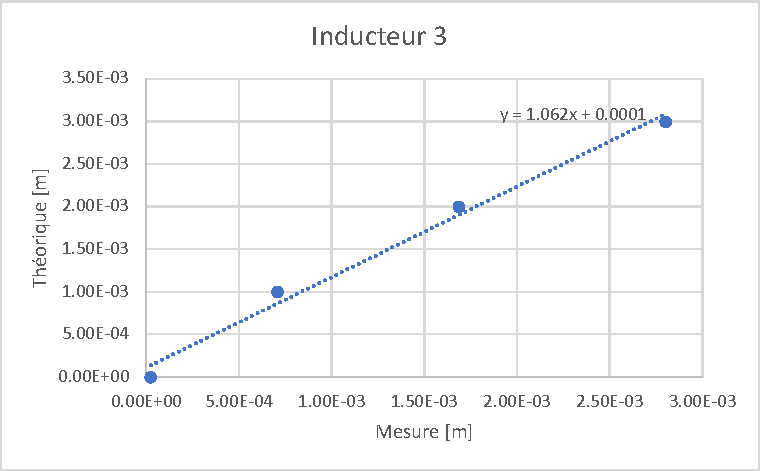
\includegraphics[width=1\linewidth]{assets/Chap3/SecEtaloInd3.pdf}
    \caption{Graphique du second étalonnage de l'inducteur 1}
    \label{fig:Sec_tracé_ind3}
\end{figure}

\begin{figure}[H]
    \centering
    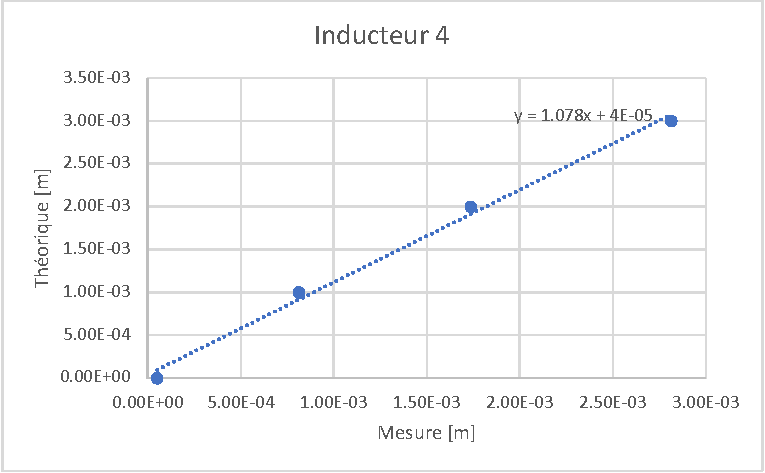
\includegraphics[width=1\linewidth]{assets/Chap3/SecEtaloInd4.pdf}
    \caption{Graphique du second étalonnage de l'inducteur 1}
    \label{fig:Sec_tracé_ind4}
\end{figure}

Après intégration de ces nouvelles équations dans le code source, une mesure de vérification a été effectuée. Les résultats sont présentés dans le tableau \ref{tab:verif_etalonnage_teachin_adc} :

\begin{table}[H]
    \centering
    \begin{tabular}{|c|c|c|c|c|}
        \hline
        \multicolumn{5}{|c|}{\textbf{Mesure des positions entrefers après l'ADC}}                     \\ \hline
        Inducteur          & Théorique {[}m{]} & Mesure {[}m{]} & Erreur   & Erreur relative {[}\%{]} \\ \hline
        \multirow{4}{*}{1} & 0.00E+00          & 1.06E-04       & 1.06E-04 & -                        \\ \cline{2-5}
                           & 1.00E-03          & 7.90E-04       & 2.10E-04 & 21                       \\ \cline{2-5}
                           & 2.00E-03          & 1.82E-03       & 1.85E-04 & 9.25                     \\ \cline{2-5}
                           & 3.00E-03          & 3.01E-03       & 1.10E-05 & 0.367                    \\ \hline
        \multirow{4}{*}{2} & 0.00E+00          & 9.30E-05       & 9.30E-05 & -                        \\ \cline{2-5}
                           & 1.00E-03          & 9.21E-04       & 7.90E-05 & 7.9                      \\ \cline{2-5}
                           & 2.00E-03          & 1.89E-03       & 1.06E-04 & 5.3                      \\ \cline{2-5}
                           & 3.00E-03          & 3.03E-03       & 2.80E-05 & 0.933                    \\ \hline
        \multirow{4}{*}{3} & 0.00E+00          & 1.38E-04       & 1.38E-04 & -                        \\ \cline{2-5}
                           & 1.00E-03          & 7.88E-04       & 2.12E-04 & 21.2                     \\ \cline{2-5}
                           & 2.00E-03          & 1.83E-03       & 1.74E-04 & 8.70                     \\ \cline{2-5}
                           & 3.00E-03          & 3.02E-03       & 1.50E-05 & 0.500                    \\ \hline
        \multirow{4}{*}{4} & 0.00E+00          & 1.16E-04       & 1.16E-04 & -                        \\ \cline{2-5}
                           & 1.00E-03          & 9.06E-04       & 9.40E-05 & 9.40                     \\ \cline{2-5}
                           & 2.00E-03          & 1.91E-03       & 8.70E-05 & 4.35                     \\ \cline{2-5}
                           & 3.00E-03          & 3.07E-03       & 7.30E-05 & 2.43                     \\ \hline
    \end{tabular}
    \caption{Mesure des positions en sortie de l'ADC (vérification de l'étalonnage après recalibration teach-in des 4 capteurs)}
    \label{tab:verif_etalonnage_teachin_adc}
\end{table}

Cependant, comme observé précédemment, ce nouvel étalonnage n'a pas permis d'améliorer la stabilité de la lévitation en conditions de fonctionnement.